\subsection{Larger tables---Overall analysis}\label{sec:twoway-overall}
For two-way tables overall tests of association can be carried out
using \PROC{FREQ}.
If the table has more than two factors (as in the
Arthritis Treatment data), the other factors will be
ignored (and collapsed) if not included the
\texttt{TABLES} statement.
This simplified analysis may be misleading if
the excluded factors interact with the factors used in the
analysis.

\begin{Example}[arthrit2]{Arthritis treatment}
Since the main interest is in the relation between treatment and
outcome, an overall analysis (which ignores sex) could be carried out
using \PROC{FREQ} as shown below.
\ixd{arthritis treatment}

\begin{listing}
title 'Arthritis Treatment: PROC FREQ Analysis';
data arth;
   input sex$ treat$ @;
   do improve = 'None  ', 'Some', 'Marked';
      input count @;
      output;
      end;
datalines;
Female  Active    6  5  16
Female  Placebo  19  7   6
Male    Active    7  2   5
Male    Placebo  10  0   1
;
*-- Ignoring sex;
proc freq order=data;
   weight count;
   tables treat * improve / cmh chisq nocol nopercent;
   run;
\end{listing}

In this analysis, note that:
\begin{itemize}
\item TREAT and IMPROVE are both character variables, which \PROC{FREQ}
       orders alphabetically (i.e., `Marked', `None', `Some') by
       default.  Because I want to treat the IMPROVE variable as
       ordinal, I used \texttt{order=data} on the \PROC{FREQ}
       statement to have the levels of IMPROVE ordered by their order
       of appearance in the \Dset.

\ix{Cochran-Mantel-Haenszel tests|(}
\item The \opt{chisq}{FREQ} gives the usual \(\chi^2\) tests
       (Pearson, Fisher's, etc.).  The \opt{cmh}{FREQ} requests the
       \IX{Cochran-Mantel-Haenszel tests}, including specialized
		 tests for ordinal variables.
\end{itemize}
The output, shown in \outref{out:arthfreq.1}, begins with the frequency table, including row
percentages.  The row percentages show a clear effect of treatment:
for people given the Active treatment, 51\% showed Marked improvement,
while among those given the Placebo, 67\% showed no improvement.

The results for the \opt{chisq}{FREQ} are also shown in \outref{out:arthfreq.1}.  All tests
show a significant association between treatment and outcome.

\begin{Output}
\caption{Arthritis treatment data, overall analysis}\label{out:arthfreq.1}
\small
\verbatiminput{ch3/out/arthfreq.1}
\end{Output}
\end{Example}

\subsection{Tests for ordinal variables}\label{sec:ordinaltests}

For \(r \times  c\) tables, different tests are applicable depending
on whether either or both of the row and column variables are
ordinal.  Tests which take the ordinal nature of a variable into
account are provided by the \opt{cmh}{FREQ} on the
\stmt{tables}{FREQ}.
These tests are based on assigning numerical scores to
the table categories;  the default (table) scores treat the levels as
equally spaced.  They generally have higher power when the pattern of
association is determined by the order of an ordinal variable.

For the arthritis data, these tests (\opt{cmh}{FREQ}) give the
output shown in \outref{out:arthfreq.2}.

\begin{Output}
\caption{Arthritis treatment data, overall analysis}\label{out:arthfreq.2}
\small
\verbatiminput{ch3/out/arthfreq.2}
\end{Output}

The three types of tests differ in the types of departure from
independence they are sensitive to:

\begin{itemize}
\item \boldital{General Association}.  When the row and column
       variables are both nominal (unordered) the only alternative
       hypothesis of interest is that there is \emph{some} association
       between the row and column variables.  The CMH test statistic
       is similar to the (Pearson) Chi-Square and Likelihood Ratio
       Chi-Square in the Statistics table; all have \((r - 1) (c -
       1)\) df.
\ix{Cochran-Mantel-Haenszel tests!general association}
\ix{likelihood ratio test}

\item \boldital{Row Mean Scores Differ}.  If the column variable is
       ordinal, assigning scores to the column variable produces a
       mean for each row.  The association between row and column
       variables can be expressed as a test of whether these means
       differ over the rows of the table, with \(r - 1\) df.  This
       is analogous to the Kruskal-Wallis non-parametric test (ANOVA
       based on rank scores).
\ix{Kruskal-Wallis test}
\ix{Cochran-Mantel-Haenszel tests!row means differ}

\item \boldital{Nonzero Correlation (Linear association)}.  When {\bf both} row and
       column variables are ordinal, we could assign scores to both
       variables and compute the correlation ($r$).  The Mantel-Haenszel
       \(\chi^2\) is equal to \(( N - 1) r^2\), where N is the total
       sample size.  The test is most sensitive to a pattern where
       the row mean score changes linearly over the rows.
\end{itemize}
\ix{Cochran-Mantel-Haenszel tests!linear association}
{\bf Notes}:

\begin{itemize}
\item Different kinds of scores can be assigned using the
\opt{scores}{FREQ}
on the \stmt{tables}{FREQ}, but only the
relative spacing of the scores is important.
The default, \pname{SCORES=TABLE} uses integer row and column numbers
for character variables, and numeric levels (or formatted equivalents)
for numeric variables.

\item When only one variable is ordinal, make it the {\bf last} one
       on the \stmt{tables}{FREQ}, because \PROC{FREQ} only computes
       means across the column variable.
\item When there are only $r=2$ rows (as there are here), the 
nonzero correlation and row
       means tests are equivalent.
		 In a $2 \times 2$ table, all three tests are identical.
\end{itemize}

\subsection{Sample CMH Profiles}\label{sec:Sample}

Two contrived examples may make the differences among these tests
more apparent.  Visualizations of the patterns of association
reinforces the aspects to which the tests are most sensitive.

\subsubsection{General Association}
\ix{Cochran-Mantel-Haenszel tests!general association|(}
The table below exhibits a
general association between variables $A$ and $B$, but no difference in
row means or linear association.  The row means are calculated by
assigning integer scores, $b_i = i$ to the column categories.
\figref{fig:cmhdemo}(a) shows
the pattern of association in this table graphically, as a sieve diagram
(described in \secref{sec:twoway-sieve}).

 \begin{center}
 \begin{tabular}{r|rrrrr|rr}
  \hline
   & b1 & b2 & b3 & b4 & b5 & Total & Mean \\ 
  \hline
  a1 & 0 & 15 & 25 & 15 & 0 & 55 & 3.0 \\ 
  a2 & 5 & 20 & 5 & 20 & 5 & 55 & 3.0 \\ 
  a3 & 20 & 5 & 5 & 5 & 20 & 55 & 3.0 \\ 
  \hline
  Total & 25 & 40 & 35 & 40 & 25 & 165 & 3.0\\ 
  Mean & 2.8 & 1.6 & 1.4 & 1.6 & 2.8 & 2.1\\
  \hline
 \end{tabular}
 \end{center}


This is reflected in the \PROC{FREQ} output shown in
\outref{out:cmhdemo.1}.
The chi-square values for non-zero correlation and different
row mean scores are exactly zero because the row means are all equal.
Only the general association test shows that $A$ and $B$
are associated.
\begin{Output}[ht]
\caption{General Association example: CMH tests}\label{out:cmhdemo.1}
\small
\verbatiminput{ch3/out/cmhdemo.1}
\end{Output}
\ix{Cochran-Mantel-Haenszel tests!general association|)}

\subsubsection{Linear Association}
\ix{Cochran-Mantel-Haenszel tests!linear association|(}
The table below contains a weak,
non-significant general association, but significant row mean
differences and linear associations.
The unstructured test of general association would therefore
lead to the conclusion that no association exists, while the
tests taking ordinal factors into account would conclude otherwise.
Note that the largest frequencies
shift towards lower levels of $B$ as the level of variable $A$ increases.
See \figref{fig:cmhdemo}(b) for a visual representation of this pattern.

 \begin{center}
 \begin{tabular}{r|rrrrr|rr}
  \hline
     & b1 & b2 & b3 & b4 & b5 & Total & Mean \\ 
  \hline
  a1 & 2 & 5 & 8 & 8 & 8 & 31 & 3.48 \\ 
  a2 & 2 & 8 & 8 & 8 & 5 & 31 & 3.19 \\ 
  a3 & 5 & 8 & 8 & 8 & 2 & 31 & 2.81 \\ 
  a4 & 8 & 8 & 8 & 5 & 2 & 31 & 2.52 \\ 
  \hline
  Total & 17 & 29 & 32 & 29 & 17 & 124 & 3.00 \\ 
  Mean & 3.1 & 2.7 & 2.5 & 2.3 & 1.9 & 2.5\\
  \hline
 \end{tabular}
 \end{center}


Note that the \(\chi^2\)-values for the row-means and non-zero
correlation tests in \outref{out:cmhdemo.2}
are very similar, but the correlation test is more
highly significant since it is based on just one degree of
freedom.

\begin{Output}[htb]
\caption{Linear Association example: CMH tests}\label{out:cmhdemo.2}
\small
\verbatiminput{ch3/out/cmhdemo.2}
\end{Output}

The differences in sensitivity and power among these tests is
analogous to the difference between general ANOVA tests and tests for
linear trend in experimental designs with quantitative factors:
The more specific test has greater power, but is sensitive to
a narrower range of departure from the null hypothesis.


%% two subfig side-by-side
\begin{figure}[htb]
 \begin{minipage}[b]{.49\linewidth}
  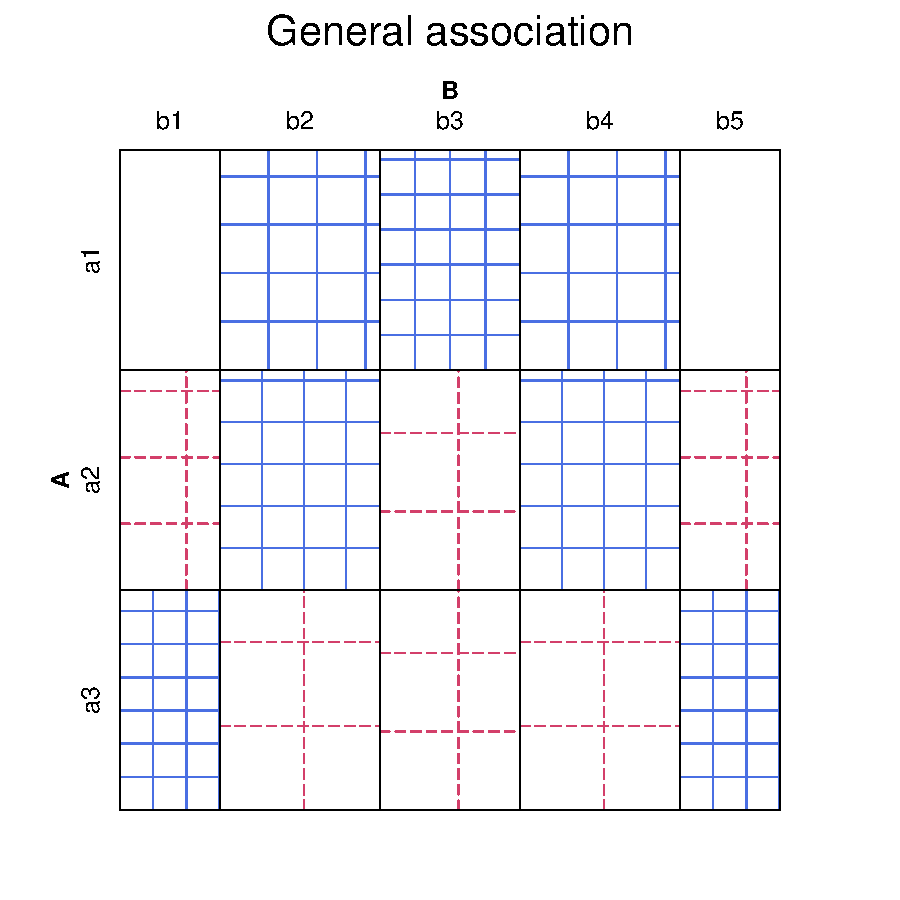
\includegraphics[width=1\linewidth]{ch3/fig/cmhdemo1}
 \end{minipage}%
 \hfill
 \begin{minipage}[b]{.49\linewidth}
  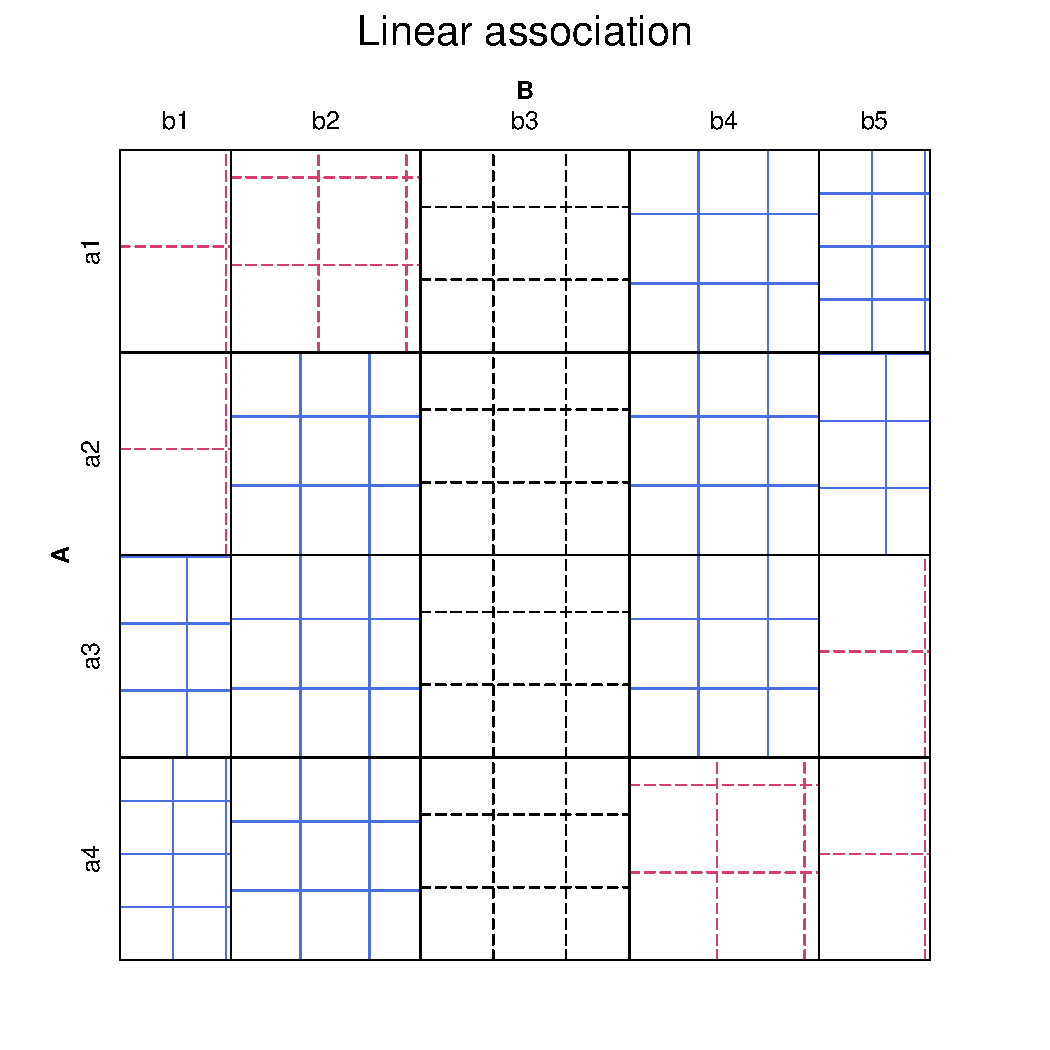
\includegraphics[width=1\linewidth]{ch3/fig/cmhdemo2}
 \end{minipage}
 \caption[Sieve diagrams for general association and linear association]{Sieve diagrams for two patterns of association. (a) General association (b) linear association.
 In each figure,
 cells with greater than expected frequency are shown with solid, blue cross hatching and the number of boxes is proportional to the observed frequency.}\label{fig:cmhdemo}
\end{figure}
\ix{Cochran-Mantel-Haenszel tests!linear association|)}
\ix{Cochran-Mantel-Haenszel tests|)}
